%\documentclass{article}
\documentclass[twocolumn]{article}
%% Language and font encodings
\usepackage[english]{babel}
\usepackage[utf8x]{inputenc}

\usepackage{booktabs}
\usepackage{tabu}
\usepackage[T1]{fontenc}
\usepackage[section]{placeins}
%% Sets page size and margins
\usepackage[a4paper,top=3cm,bottom=3cm,left=3cm,right=3cm,marginparwidth=3cm]{geometry}


%% Useful packages
\usepackage{amsmath}
\usepackage{amsfonts}
\usepackage{graphicx}
%\usepackage{apacite}
\usepackage[colorinlistoftodos]{todonotes}
\usepackage[colorlinks=true, allcolors=blue]{hyperref}

\usepackage{titlesec}
\titleformat{\section}[block]{\filcenter}{}{1em}{}
\titleformat*{\section}{\LARGE\bfseries\center}
\titleformat*{\subsection}{\Large\bfseries}
\titleformat*{\subsubsection}{\large\bfseries}
\titleformat*{\paragraph}{\large\bfseries}
\titleformat*{\subparagraph}{\large\bfseries}


\begin{document}
	\begin{titlepage}
		\begin{center}
			\vspace*{1cm}
			\Huge
			\textbf{Transfer Learning in Deep Reinforcement Learning}
					
			\vspace{1.5cm}
			\Large
			Author: \textbf{David Liang}\\
			
			Advisor: \textbf{Professor Yu Hen Hu}
			
			\vfill
			
			A thesis presented for \\
			Undergraduate Honors in Computer Sciences
			
			\vspace{0.8cm}
			
\includegraphics[width=0.5\textwidth]{university}
			
			
			\Large
			Department of Computer Sciences\\
			University of Wisconsin-Madison\\
			United States\\
			5/10/2018
		\end{center}
	\end{titlepage}

	\twocolumn[
	\begin{@twocolumnfalse}
		\begin{abstract}
			\normalsize
			\centering\begin{minipage}{\dimexpr\paperwidth-10cm}
			Reinforcement learning has quickly risen in popularity because of 
			its simple, intuitive nature and it's powerful results. In this 
			paper, we study a number of reinforcement learning algorithms, 
			ranging from asynchronous q-learning to deep reinforcement 
			learning. We focus on the improvements they provide over standard 
			reinforcement learning algorithms, as well as the impact of initial 
			starting conditions on the performance of a reinforcement learning 
			agent.\\\\
			\end{minipage}
		\end{abstract}
	\end{@twocolumnfalse}
	]
		
	\section{Introduction} 
	Reinforcement learning is a class of machine learning algorithms that 
	are designed to allow agents provided with only the knowledge of the states 
	it visits and the actions available to the agent to learn how to maximize 
	its reward function, quite similar to the trial-and-error 
	approach~\cite{Kaebling}. There are different techniques used for 
	reinforcement learning, one of the most popular ones being 
	``Q-learning''~\cite{Watkins} where an agent develops a policy that chooses 
	the action that is estimated to lead to the greatest total future rewards. 
	Reinforcement learning has seen great recent success, particularly in 
	``Playing Atari with Deep Reinforcement Learning'' ~\cite{Mnih} and 
	``Mastering Chess and Shogi by Self-Play with a General Reinforcement 
	Learning Algorithm''~\cite{Silver} (AlphaZero) as it is a relatively simple 
	yet extremely powerful algorithm, making it an interesting class of 
	learning algorithms to study. Furthermore, the training of reinforcement 
	learning agents is extremely slow, since the information it is provided is 
	minimal, which means that there is a lot of room for improvement with 
	reinforcement learning algorithms. Transfer learning on the other hand is a 
	class of machine learning algorithms that seeks to transfer ``knowledge'' 
	gained from solving one problem and applying it to another problem, so 
	transfer learning can solve the problem of speed for reinforcement learning 
	agents. In this paper, we discuss the impact of initial conditions with 
	transfer learning on the convergence of reinforcement learning 
	agents.\\	

	
	\section*{Motivation}
	In real life, we know that initial starting conditions matter. Consider a 
	person who chooses to learn a sport: the athletic ability, age, equipment, 
	training, and instructor will all influence the time it takes for the 
	person's skill to peak. If it were at all possible, we would want to 
	transfer the traits of high-performing athletes to the beginner to provide 
	better chances at performing well. Based on this intuition, we 
	want to experiment with transferring the models of trained reinforcement 
	learning agents as the initial starting conditions of reinforcement 
	learning algorithms and confirm that this hypothesis does indeed apply here 
	too. That is, we want to show that given ``better'' initial conditions, an 
	agent will likely achieve high performance faster than an agent with 
	``worse'' initial conditions. This is reasonable, and we can easily produce 
	simple examples that illustrate the point. Consider an extreme example 
	where an agent uses a neural network to model its policy, and all the 
	weights in the network are initialized to zero. Then all the weights follow 
	the same gradients, and the policy will likely perform poorly. Conversely, 
	an agent with a policy model that has been trained for extremely long 
	periods of time will likely be much closer to optimality: hence it will 
	likely take much less time to converge. Intuitively, it makes sense that 
	better initial conditions lead to optimal performance faster, and we wish 
	to establish this for reinforcement learning, by means of a simple form of 
	transfer learning. \\
	
	
	\section*{Background}
	\subsubsection*{Reinforcement Learning}
	The reinforcement learning task is often formulated as a Markov decision process, a modeling framework useful for partially random, partially controlled environments, which is certainly the case in reinforcement learning where the environment may behave randomly, but the agent has control over its own actions. In the reinforcement learning task, a Markov decision process consists of the following elements:
	\begin{enumerate}
		\item $S_E$: The set of states that the environment (with the agent in it) $E$ can be in. 
		\item $A_E$: The set of possible actions that the agent can take in the environment.
		\item $W_E:S_E \times A_E \to S_E$: The function that determines the resulting state given a starting state and an action.
		\item $R_E:S_E \times S_E \to \mathbb{R}$: The function that gives the immediate reward for a state transition.		
	\end{enumerate}
	The agent constructs a policy $\pi_E:S_E \to A_E$ that maps a state in the 
	state space to an available action that leads to the highest total 
	immediate and future rewards. But because future rewards are 
	not easily estimated in stochastic environments, a discount rate $\gamma$ 
	is introduced for future rewards so that given the choice between one 
	immediate or one future reward (both equal in value), it will choose the 
	immediate reward because of the stochastic environment. So we formulate a 
	utility function $U_{\pi_E}:S_E\to \mathbb R$ that determines all rewards 
	received by following the policy given a starting point $s_0$: 
	$$U_{\pi_E}(s_0) = \sum_{t=0}^\infty \gamma^t R_E(s_t, 
	W_E(s_t,\pi_E(s_t)))$$ 	Then the policy for our reinforcement learning 
	agent can be defined as follows: 
	$$\pi_E(s_t) = \text{argmax}_{a \in A_E}U_{\pi_E}(W_E(s_t, a))$$\\
	
	\subsubsection*{Q-learning}
	Often times, an agent does not have access to $W_E$ and in such cases, the 
	agent's policy is said to be ``model-free.'' The agent must, then, estimate 
	the utility function by it's internal Q-value function $Q_{\pi_E}: S_E \to 
	\mathbb R$. A simple way to represent $Q_{\pi_E}$ is to use a table in 
	which each possible state and action pair is listed, and the estimated 
	cumulative reward is the entry. To learn the optimal Q-value function 
	which we denote by $\hat{Q}_E$, we use the Q-learning algorithm on our 
	Q-value function $Q_{\pi_E}$. In one-step Q-learning, the algorithm takes 
	one step at every training iteration $t$ from state $s_t$, observes the 
	reward received $r_t$ 	and the new state $s_{t+1}$, and updates the policy 
	as follows: $$Q_{\pi_E}(s_t) = Q_{\pi_E}(s_t) + \alpha(r + \gamma 
	Q_{\pi_E}(s_{t+1}) - Q_{\pi_E}(s_t))$$ with $\alpha$ as the learning rate, 
	typically a real number between $0$ and $1$. This algorithm sets the target 
	value to be the discounted sum of all the future rewards estimated by 
	$\gamma Q_{\pi_E}(s_{t+1})$ added to the observed immediate reward $r$. The 
	difference between the target value and output value is then a weighted by 
	the learning rate, and used to update the Q-function. To avoid settling for 
	a non-optimal policy (premature convergence of policy), an exploration 
	factor $\epsilon$ is introduced: $\epsilon$ is the probability that the 
	agent will ignore its policy and execute a random action, to diversify its 
	experiences and to avoid local minima in its policy. As time progresses, 
	the exploration rate is decayed, so that the agent relies more (but not 
	completely) on its policy. However, it is often the case that the 
	exploration rate is not allowed to decay to $0$ and is instead held at some 
	fixed minimum exploration rate, to discourage the policy from sinking into 
	a local minimum.\\
	
	\subsubsection*{Q-networks}
	It becomes hard to maintain such a Q-table when the size of the state space 
	increases: for example, consider an agent playing a video game, using the 
	screen's pixel values as its state space. If the state is a $84 \times 84 
	\times 3$ array of $8$ bit pixels and there are four actions available, the 
	q-value table will hold $2^{84*84*3+2} \approx 10^{6351}$ entries! A 
	popular solution to the problem of poorly scaling tables is the use of 
	artificial neural networks in Q-learning termed Q-networks. 
	Q-networks map states in the state space, represented by frames from the 
	game, to q-values for each possible action. Q-networks learn to approximate 
	$\hat{Q}$ in a way intuitively similar to the update formula for the 
	Q-table, by computing gradients for the network based on the output of the 
	network (determined without knowing the next states) and target Q-values 
	(determined using the next states) for the network. Q-networks are far more 
	powerful than Q-tables because they can also approximate Q-values for 
	states it has not yet seen and scales much better in terms of size. 
	However, they come with the downside of being harder and slower to 
	train.\\
	
	\subsubsection*{Convolutional Neural Networks}
	One particular class of neural networks that has seen great success with 
	images is the convolutional neural network (CNN), used for the task of 
	image 	
	classification~\cite{Krizhevsky}~\cite{Zeiler}~\cite{Simonyan}~\cite{Szegedy}.
	Part of its success is due to the fact that each layer can contain fewer 
	weights, allowing for faster training. Each set of weights in a particular 
	layer can be seen as a filter that is applied over the input image. A set 
	of weights can then learn to detect certain features in each image of the 
	input, and subsequent layers can learn mappings from these features to new 
	features. A CNN also subsamples between layers to reduce the dimensionality 
	of the image input, and is usually completed by a set of densely connected 
	layers, the same as those found in the artificial neural network. \\
	
	\subsubsection*{Deep Reinforcement Learning}
	With the above features, CNNs have become immensely popular, and lots of 
	work has been done to apply CNNs to other fields. In particular, CNNs have 
	been applied extremely successfully to reinforcement Q-learning, perhaps 
	most notably in the deep Q-network 	(DQN)~\cite{Mnih}~\cite{Mnih2}. This 
	research has introduced a number of improvements. First, states are 
	provided to the DQN agent as a sequence of frames, not just one. This 
	provides temporal knowledge to the agent, which has proven to be 
	beneficial. Then in order to combat the highly correlated data that comes 
	from online learning, ``experience replay'' is introduced. This feature 
	essentially stores a tuple of a state, the action taken from the 
	state, the reward incurred for the action, and the
	resulting state from the action, termed an ``experience.'' In training, the 
	experiences are randomly sampled and used for training the network. To 
	improve the stability of the learning algorithm, every $C$ updates, the 
	network $Q_{\pi_E}$is cloned to obtain a target network 
	$\tilde{Q}_{\pi_E}$, which is used to compute the Q-value targets. The 
	gradients obtained are then applied to $Q_{\pi_E}$, not 
	$\tilde{Q}_{\pi_E}$. Hence this less-frequently updated target network 
	gives more stable gradients, leading to more stable learning. \\
	
	\subsubsection*{Transfer Learning}
	As discussed before, it is well known that reinforcement learning can be 
	slow, and in fact, one may end up running the same training algorithm for 
	different environments, regardless of similarity in task, incurring an 
	increase in training time linearly proportional with the number of 
	environments. As such, it would be advantageous if one model could be 
	trained and have its knowledge transferred to the other 	
	models~\cite{Taylor}~\cite{Fang}~\cite{Wei}~\cite{Yin}. This is the 
	intuition behind transfer learning. Transfer learning gets quite 
	complicated when it comes to determining what to transfer and how to 
	transfer it. A simple example of transfer learning can be observed by 
	training the agent to solve all of the subtasks that compose a single 
	master task. This effectively allows the agent to complete the master task 
	where it can be presented with any of the subtasks. In our particular case, 
	we transfer the model of a pre-trained DQN agent to a beginning DQN agent 
	and study its training with this initial condition.\\
	
	
	\section*{Related work} 
	\subsubsection*{Asynchronous Q-learning}
	An interesting improvement to Q-learning is asynchronous Q-learning (AQL). 
	This technique involves one central, shared neural network. Then each 
	asynchronous agent copies the shared network as its own individual 
	network, learns on its own, and periodically shares its accumulated updates 
	(gradients) with the shared neural network. Furthermore, each agent will 
	periodically copy the shared neural network as it's own individual neural 
	network, making use of the learning that other agents have done. In effect, 
	an AQL agent searches across multiple locations in the state space while 
	sharing information with other agents, speeding up its learning process 
	\cite{Mnih3}. Another effect of AQL is that local minima are more easily 
	avoided. This is due to the fact that there are multiple agents in 
	different locations of the state space: an agent in a local minima can be 
	pulled out when it copies in the shared neural network. Similarly, the 
	shared neural network can be pulled out of a local minima when other agents 
	share its updates with the shared neural network. Finally, AQL gives the 
	improvement of CPU computation being more efficient than GPU computation, 
	which is monetarily expensive \cite{Mnih3}. As such, we see that AQL is a 
	highly effective improvement to Q-learning.\\

	
	\section*{Approach} 
	We first describe the infrastructure available to us for our experiments. 
	For high numbers of independent experiments, we use a distributed 
	high-throughput computing resource through the Center for High Throughput 
	Computing (CHTC) available at UW-Madison. As a result, we can run many 
	independent experiments with lots of hardware resources, but we don't have 
	GPU access,	so training on CHTC is quite slow. 	For our asynchronous 
	training experiment, we use OpenAI's ``FrozenLake-v0'' environment and 
	consider the task to be solved when a win-rate of $78\%$ is achieved, as 
	defined by OpenAI. For our guaranteed convergence experiment, we tested 
	using a custom maze environment with a state size of $4$ and an action 
	space size of $4$. For our initial conditions experiment, we describe how 
	we define an operational convergence criteria for our problem setting. We 
	say that the agent's learning has stopped if the winning rate over the last 
	$100$ evaluations averages to a value greater than $.78$, the same stopping 
	criteria for the environment FrozenLake.\\
	
	
	\section*{Experiments} 
	We conducted a number of experiments to study the state-of-the-art in 
	reinforcement learning and to try to answer our initial questions. We 
	present them below, describing our motivation and the results. Code for 
	these experiments can be found in our 
	\href{https://github.com/dliangsta/RL-thesis}{Github repository}.\\
	
	\subsubsection*{Asynchronous Training}
	We know from Mnih et al.\cite{Mnih3} that asynchronous q-learning improves 
	training speeds. Our hypothesis here was that an asynchronous q-network 
	would 
	provide faster training times (in terms of training epochs), proportional 
	to the number of asynchronous agents used. Our hypothesis was affirmed by 
	our experiment  as seen in figure \ref{fig:AQL-Iterations}. It is worth 
	noting, though, that our experiments were not run over a distributed 
	computing system: instead, each agent was run on a single CPU, meaning that 
	the total training times (in terms of pure time) were similar 
	as shown in figure \ref{fig:AQL-Time}. We are confident that running the 
	network over a 	large distributed system provide training times inversely 
	proportional to the number of agents used because of the inversely 
	proportional change in iterations per agent. When running each agent on a 
	separate core/cluster, these improvements in training time can be 
	achieved. This experiment was conducted on a system with an Intel i7-7700k 
	with 32 GB DDR4 3200 MHz SDRAM on a Samsung 960 EVO M.2 drive.\\
	\begin{figure*}[!htb]
		\centering
		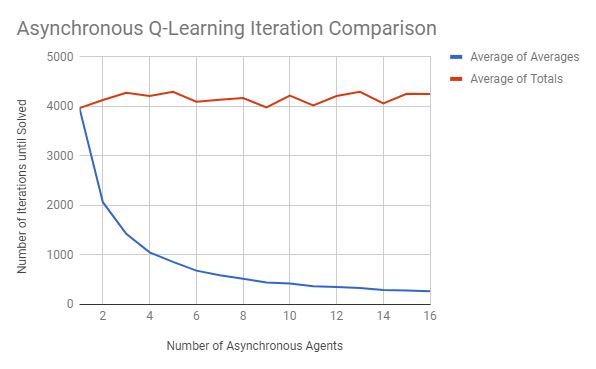
\includegraphics[width=\linewidth]{AQL-Iterations.JPG}
		\caption{Comparison of average total number of iterations over all 
		agents until the task was solved and the average of the number of 
		iterations of each agent.}
		\label{fig:AQL-Iterations}
	\end{figure*}\\
	\begin{figure*}[!htb]
		\centering
		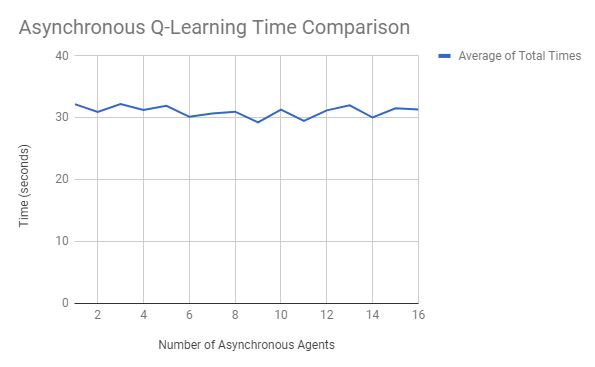
\includegraphics[width=\linewidth]{AQL-Time.JPG}
		\caption{Comparison of average total time over all agents until the 
		task was solved.}
		\label{fig:AQL-Time}
	\end{figure*}\\
	
	\subsubsection*{Guaranteed Convergence Given Infinite Time}
	We know from Even-Dar et. al\cite{Even-Dar} that using the 
	action-elimination algorithm, 
	our reinforcement learning agent will converge given infinite time. Our 
	hypothesis was that the algorithm would work for a reinforcement learning 
	agent in an environment with an extremely simple problem with an extremely 
	small state space. We expected to see the algorithm converge given a couple 
	months time. Unfortunately, the algorithm's progress exponentially 
	diminished, and we never saw the convergence (or anything even close) after 
	2 months of running the algorithm on a high-throughput computing cluster. 
	As such, we affirm that ``infinite time'' really does mean some enormous 
	time quantity that is infeasible. We ran this experiment on a Google Cloud 
	Compute Engine instance with 8 cores and 32 GB RAM.\\
	\subsubsection*{Impact of Initial Conditions on Convergence}
	We hope to find that given ``better'' initial conditions, our DQN agent 
	will converge faster. We provided these initial conditions as trained DQN 
	models, saved after various periods of pre-training. We hypothesize that 
	models that have had more pre-training will require less time to converge, 
	while models that have had little pre-training. We first show the baseline 
	performances of each initial condition in figure \ref{fig:baseline}. Then 
	we show training times until convergence starting from each initial 
	condition in figure \ref{fig:convergence} (note that the experiments have 
	not yet concluded so the figure is incomplete for the time being). Our 
	hypothesis is affirmed 	through this experiment as we can see that indeed 
	agents with more pre-training had faster times to convergence. The 
	pre-training was done on a system with an Intel i7-7700k overclocked to 4.9 
	GHz with 32 GB DDR4 3200 MHz SDRAM on a Samsung 960 EVO M.2 drive. When 
	testing each initial condition, we used CHTC. Each job was run on a system 
	with 8 CPUs and 10 GB memory. Each job ran inside of a docker container.\\
	\begin{figure*}[htb]
		\centering
		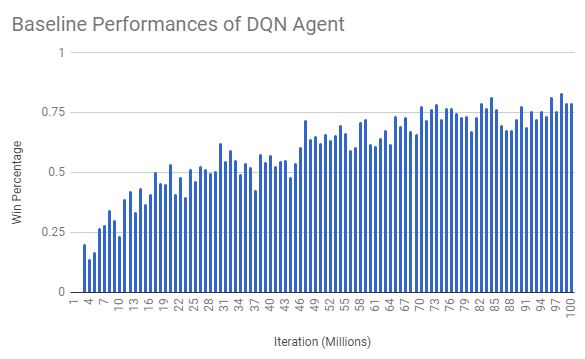
\includegraphics[width=\linewidth]{baseline.jpg}
		\caption{Baseline performances of the DQN agent. The x-axis shows the number of iterations that had passed when the agent was saved while the y-axis shows the winning percentage of the agent over 1000 games.}
		\label{fig:baseline}
	\end{figure*}\\
	\begin{figure*}[htb]
		\centering
		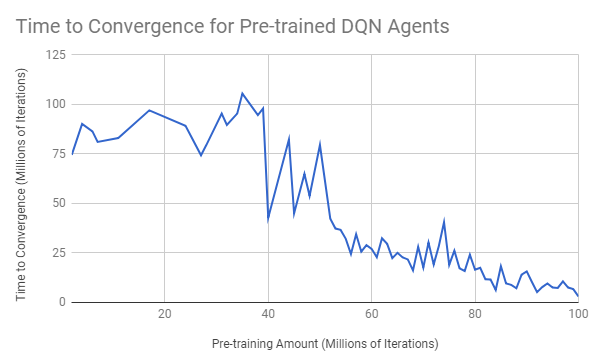
\includegraphics[width=\linewidth]{convergence.PNG}
		\caption{Comparison of time to convergence for different amounts of 
		pretraining for DQN agents.}
		\label{fig:convergence}
	\end{figure*}\\
	
	\section*{Conclusion}
	We have shown that initial conditions greatly impact the rate of 
	convergence for reinforcement learning. As a result, transfer learning 
	shows great potential for accelerating the convergence rate of 
	reinforcement learning agents. Transfer learning has already seen great 
	success in deep reinforcement learning, and we hope that this research is 
	now further motivated.\\
	
	\section*{Future Work}
	In the future, we would want to study adversarial learning in the 
	reinforcement learning setting~\cite{Lin}. Intuitively, presenting 
	challenges allows humans to learn better, and we believe that this 
	translates to reinforcement learning agents as well. In fact, it has 
	already been shown that this adds robustness~\cite{Pinto}. Furthermore, 
	adversarial learning is 
	perfectly suited for two-player games like many of the Atari games. Hence 
	our future work should include studies in adversarial learning in the 
	reinforcement learning setting. We would also like to study learning models 
	for multiple games and using transfer learning to apply these models to 
	different reinforcement learning tasks.\\

	\bibliographystyle{plain}
	\bibliography{refs}{}
	
\end{document}